% Chapter 3

\chapter{PROPOSED METHODOLOGY}\label{cha:method}

The whole system rests on one design decision: Pareto front construction (Tier~1) is
kept apart from route selection (Tier~2). The front depends on the region and the
weather, so it is built once per delivery region and refreshed when it goes stale. The
choice of route depends on the payload, so it is made per mission, against whatever
front is current. A mission that arrives between refreshes runs only Tier~2, which
reads the payload tags and returns a route in a fraction of a millisecond.

Figure~\ref{fig:methodology} gives an overview of the workflow, from environment data
to the flown mission, with baseline planners and an evaluation module scoring each
stage.

\begin{figure}[!htbp]
\centering
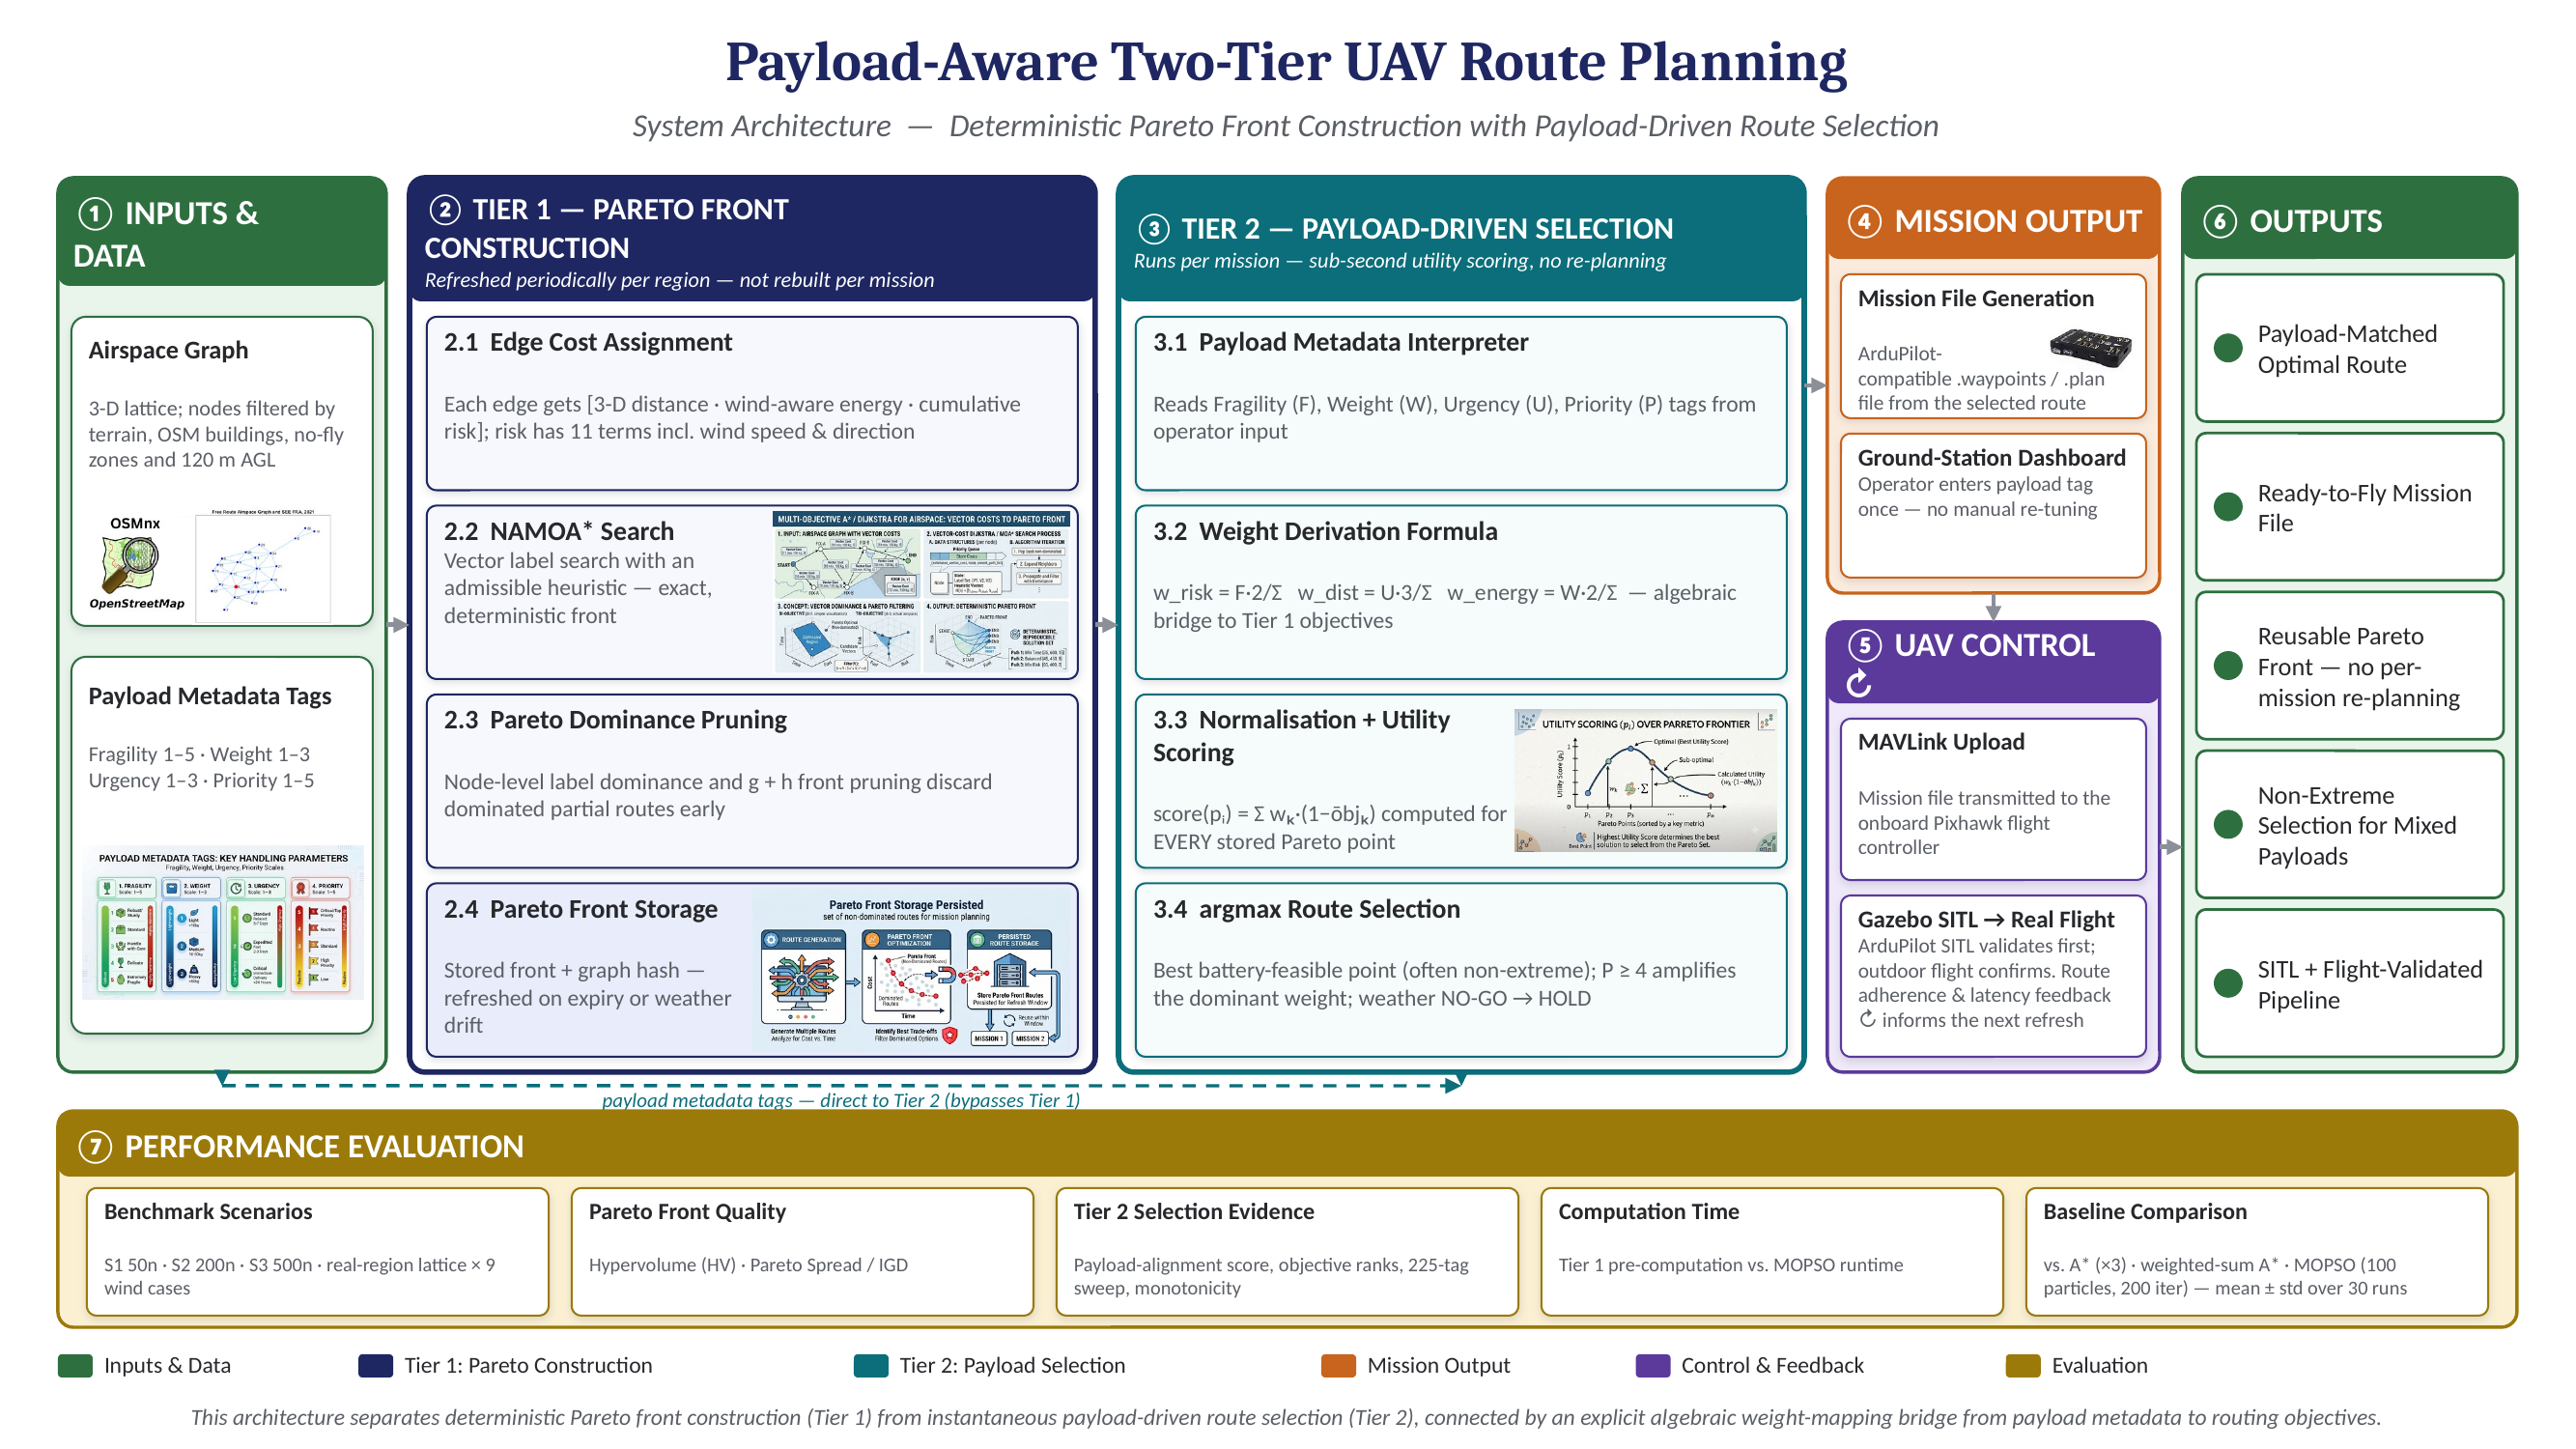
\includegraphics[width=\textwidth]{images/methodology.png}
\caption{Methodology overview: Tier~1 Pareto front construction feeding Tier~2
payload-aware route selection, with mission output, UAV control and evaluation}
\label{fig:methodology}
\end{figure}

\section{ARCHITECTURE DESIGN}\label{sec:arch}

Figure~\ref{fig:architecture} shows the system architecture, which has five layers.
The environment data layer fetches weather, terrain and OpenStreetMap layers and caches
them on disk, so that a network failure falls back to the last good copy instead of
stopping the planner. Module~1 turns these layers into a directed airspace graph whose
edges carry a three-objective cost vector. Tier~1 (Module~2) computes the Pareto front
over that graph and keeps it in a front store, together with what is needed to decide
when it is stale. Tier~2 (Module~4) reads the operator's payload tags and returns one
route from the stored front, or a HOLD advisory when the weather or the battery rules
the mission out. The output layer (Modules~6 and~7) writes the mission file and flies
it in Gazebo with ArduPilot SITL. Modules~3 and~5 sit beside the main path. They run the
baseline planners and compute the quality measures used in Chapter~\ref{cha:results}.

\begin{figure}[!htbp]
\centering
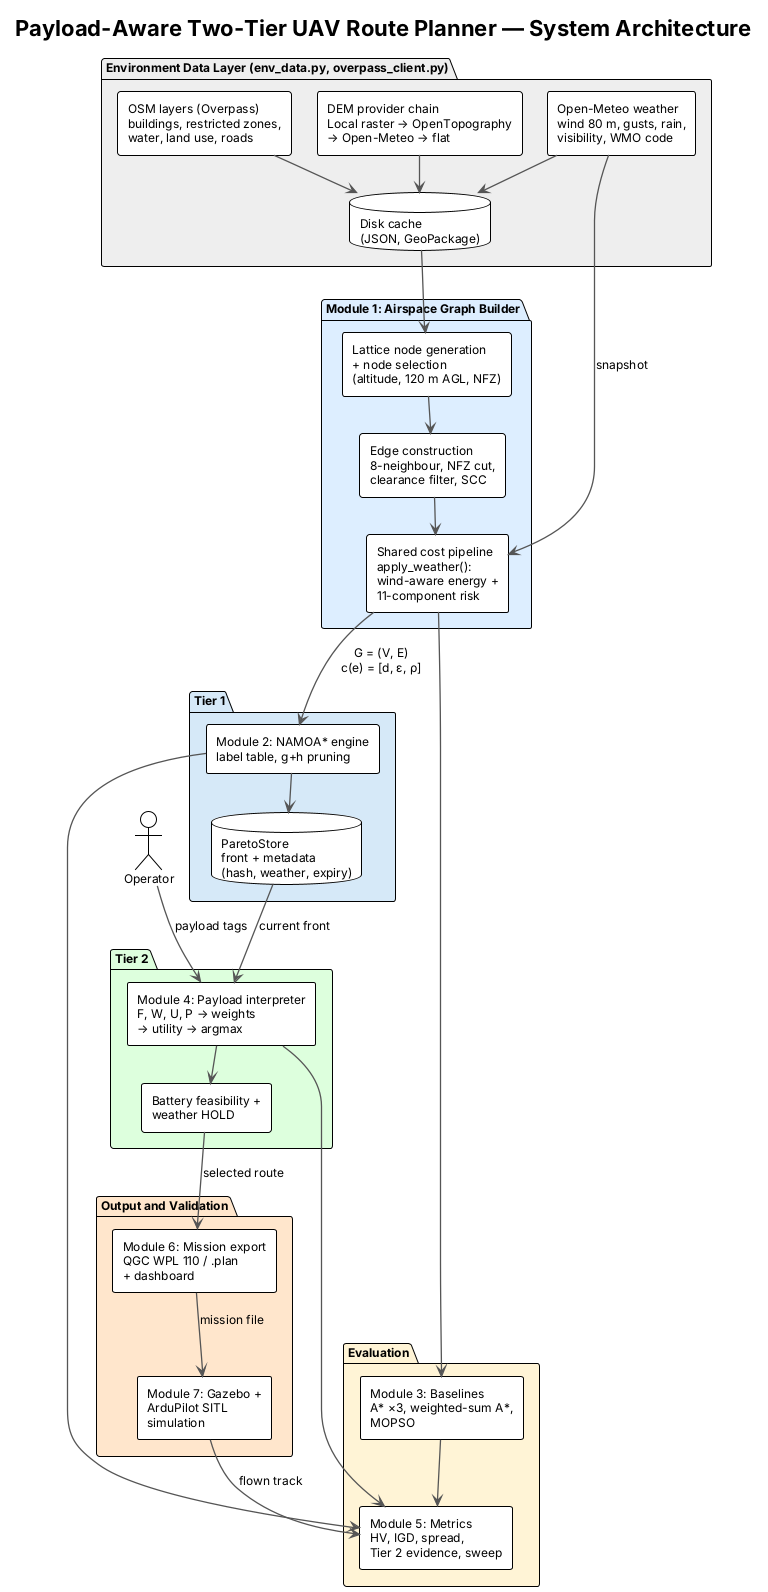
\includegraphics[width=\textwidth,height=0.30\textheight,keepaspectratio]{images/arch.png}
\caption{System architecture. Tier~1 builds and stores the front per region and
weather window; Tier~2 selects a route per payload tag; Modules~6 and~7 export and fly
it}\label{fig:architecture}
\end{figure}

Every edge $e = (u, v)$ of the airspace graph carries the cost vector
\begin{equation}
  \mathbf{c}(e;\omega) = \bigl[d(e),\; \varepsilon(e;\omega),\; \rho(e;\omega)\bigr]
\end{equation}
where $d(e)$ is the three-dimensional length of the segment in kilometres,
$\varepsilon(e;\omega)$ is the wind- and grade-aware energy proxy and $\rho(e;\omega)$
is the cumulative risk exposure along the segment under weather snapshot $\omega$.
Section~\ref{sec:m1} defines all three. The three objectives are to minimise distance,
energy and risk. Route $p$ dominates route $q$, written $p \prec q$, when $p$ is no
worse than $q$ on all three objectives and strictly better on at least one. The Pareto
front $\mathcal{P}$ is the set of routes that no other route dominates.

The code is organised into seven modules. The numbering follows the source files, so
Module~3 holds the baselines and Module~4 holds Tier~2. The sections below describe each
module's purpose, inputs, processing and outputs.

% ------------------------------------------------------------
\section{AIRSPACE GRAPH BUILDER (MODULE 1)}\label{sec:m1}

Module~1 builds the delivery airspace graph $G = (V, E)$. Its inputs are the region
(centre, box size and lattice spacing), the environment layers described below and a
weather snapshot $\omega$. Its output is a directed NetworkX~\cite{r5} graph whose nodes
carry position and altitude and whose edges carry static features, a per-component risk
breakdown and the cost vector $[d, \varepsilon, \rho]$. The weather go/no-go state is
stored on the graph itself so that Tier~2 can read it. Two builders share one cost
pipeline: a lattice builder over a real region, described below, and a seeded synthetic
builder for controlled benchmarks (Section~\ref{sec:dataset}).
Algorithm~\ref{alg:m1} summarises the lattice builder, and the subsections that follow
give the rules behind each step.

\subsection{Environment data acquisition}

Weather comes from the Open-Meteo forecast service~\cite{r20}: the 10\,m wind, gust,
rain, visibility and WMO code, and the hourly 80\,m wind speed and direction. With no
network the last cached snapshot is used, and with no cache the planner assumes calm
air so that runs stay deterministic. Terrain comes from a chain of elevation providers
tried in order (a local GeoTIFF, OpenTopography Copernicus 30\,m, Open-Meteo elevation,
and flat ground as a last resort), each cached on disk. OpenStreetMap buildings,
restricted zones, water and land use are fetched through a multi-endpoint Overpass
client with retries, cached as GeoPackage files~\cite{r4} and indexed in a local metric
frame with Shapely STRtree structures for fast height, distance, containment and
segment-intersection queries.

\subsection{Lattice generation and node selection}

A UAV is not tied to roads, so the airspace is a regular lattice, not a road network.
The region is covered by an $n \times n$ lattice in a local equirectangular frame centred
on the region, with $n = \mathrm{round}(\mathit{box}/\mathit{spacing})$. The default
6\,km box at 200\,m spacing gives 900 candidate nodes. A candidate does not enter the
graph automatically. It has to pass a selection rule that combines four data sources: ground elevation from the DEM, the tallest building in
the node's cell, the legal ceiling and restricted airspace. For node $k$ with ground
elevation $z_k$ and tallest building $b_k$ in its cell,
\begin{equation}
  \mathrm{AGL}_k = \max\bigl(H_\mathrm{cruise},\; b_k + C\bigr), \qquad
  \mathrm{alt}_k = z_k + \mathrm{AGL}_k \label{eq:alt}
\end{equation}
with cruise height $H_\mathrm{cruise} = 60$\,m and clearance $C = 15$\,m. A building's
height is read from its \texttt{height} tag, else from \texttt{building:levels} times
3\,m, else from a default for its type. A node with $\mathrm{AGL}_k > 120$\,m is
blocked, because it cannot be flown legally under the Drone Rules, 2021~\cite{r21}. A
node inside a restricted polygon (an aerodrome, military land, a prison, a protected area
or a government site) is removed. Every surviving node stores its position in both
frames, its ground elevation, the building height, density and mean height of its cell,
its height above ground and its altitude above mean sea level.

\subsection{Edge construction and pruning}

Each surviving node is linked to its eight neighbours in both directions, so the graph
is directed from the start. Three filters then remove edges: any edge whose segment
crosses a restricted polygon, any edge rejected by the optional \texttt{edge\_filter}
hook (used by the simulation module for roof and terrain clearance), and every edge
outside the largest strongly connected component, so that all remaining nodes can reach
each other.

For each edge that survives, the module stores the horizontal haversine length $d_h$,
the forward-azimuth bearing $\theta$, the grade $g = \Delta\mathrm{alt}/d_h$ and the
three-dimensional length $d = \sqrt{d_h^2 + \Delta\mathrm{alt}^2}$.

\subsection{Static risk terms}

Static terms do not depend on the weather, so they are computed once per build. Each
edge is sampled every 25\,m along the straight line between its two endpoint
altitudes. At each sample the module knows the flight altitude, the ground height, the
tallest roof directly below and the tallest roof within 30\,m. Table~\ref{tab:risk} lists all eleven risk components,
static and weather-dependent, with the weight each carries in the edge score
\begin{equation}
  \rho_\mathrm{edge} = \operatorname{clip}\Bigl(\sum_k w_k\,\rho_k,\; 0,\; 1\Bigr),
  \qquad \rho(e;\omega) = \rho_\mathrm{edge}\cdot\frac{d_h}{s} \label{eq:risk}
\end{equation}
where $s$ is the lattice spacing. Multiplying by $d_h/s$ turns the per-edge score into
a cumulative exposure. The risk of a route therefore grows with the distance flown
through risky air.

\begin{small}
\begin{longtable}{|P{2.4cm}|P{10.6cm}|P{1.0cm}|}
\caption{Risk components (every $\rho_k \in [0,1]$) and their weights}\label{tab:risk}\\
\hline
\textbf{Component} & \textbf{Model} & $\boldsymbol{w_k}$\\
\hline
\endfirsthead
\hline
\textbf{Component} & \textbf{Model} & $\boldsymbol{w_k}$\\
\hline
\endhead
Obstacle & Seeded obstacle discs, $0.9(1 - r/R)$ inside a disc (synthetic graphs only) & 1.00\\
\hline
Building & Mean over samples of $[\text{roof within 30\,m}]\cdot\bigl(1-\operatorname{clip}(m/60)\bigr)$, $m$ = margin above that roof & 0.60\\
\hline
Terrain & $\max\bigl(1-\operatorname{clip}(m_{\min}/15),\ \operatorname{clip}(\lvert g\rvert/0.30)\bigr)$: lowest clearance margin or sudden altitude change & 0.30\\
\hline
Wind & $\operatorname{clip}(C\!W/40)$, crosswind against a 40\,km/h saturation speed & 0.30\\
\hline
Gust & $\operatorname{clip}\bigl(0.5\max(0, \mathit{gust} - v)/40\bigr)$ & 0.30\\
\hline
Weather & $0.5\operatorname{clip}(\mathit{rain}/7.5) + 0.5\operatorname{clip}(1 - \mathit{vis}/10\,\mathrm{km})$, uniform over the graph & 0.20\\
\hline
Population & Mean land-use class score along the edge (our values, ranked in the spirit of SORA~\cite{r22}): assembly 1.0, commercial 0.7, major road 0.6, residential 0.5, industrial 0.3 & 0.50\\
\hline
No-fly buffer & $\max_k \exp(-\delta_k/150\,\mathrm{m})$ to the nearest restricted zone, zero beyond 600\,m & 0.80\\
\hline
Water & Fraction of samples over water (risk of losing the payload) & 0.30\\
\hline
Comm/GPS & $\operatorname{clip}(\mathit{density}/0.30)\cdot\operatorname{clip}(\bar{h}/30\,\mathrm{m})$, urban canyon effect & 0.20\\
\hline
Turbulence & $\operatorname{clip}(\mathit{density}/0.30)\cdot\operatorname{clip}(v/40)$ & 0.20\\
\hline
\end{longtable}
\end{small}

The weights are design values that put restricted zones, buildings and crowds ahead of
the weather terms. They have not been calibrated against flight data, and calibrating
them is part of the evaluation work that remains in Phase~I.

\subsection{Wind-aware energy model}

For an edge on bearing $\theta_\mathrm{edge}$ and a wind of speed $v$ blowing from
$\theta_\mathrm{from}$ (the meteorological convention), the headwind and crosswind
components are
\begin{equation}
  H\!W = v\cos(\theta_\mathrm{edge} - \theta_\mathrm{from}), \qquad
  C\!W = v\,\lvert\sin(\theta_\mathrm{edge} - \theta_\mathrm{from})\rvert \label{eq:hwcw}
\end{equation}
A positive $H\!W$ is a headwind. The energy proxy of the edge is
\begin{equation}
  \varepsilon = d\left(1 + \lvert g\rvert + \beta_h\frac{\max(0, H\!W)}{V_c}
  + \beta_c\frac{C\!W}{V_c}\right) \label{eq:energy}
\end{equation}
with cruise airspeed $V_c = 36$\,km/h, $\beta_h = 0.40$ and $\beta_c = 0.15$. A
tailwind earns no credit. This is deliberate: it keeps $\varepsilon \geq d$ on every
edge, and the Tier~1 heuristic relies on that bound. The wind speed is the 80\,m
forecast when available, which is close to the 60--120\,m cruise band. Otherwise the
10\,m value is lifted to cruise height with the power law
\begin{equation}
  v_h = v_{10}\left(\frac{h}{10}\right)^{\alpha}, \qquad \alpha = 0.25
\end{equation}
following Peterson and Hennessey~\cite{r19}. A gust factor measured at 10\,m is applied
to the wind at flight height.

Because of Equation~(\ref{eq:hwcw}), edge costs are directional: flying $u \rightarrow
v$ and $v \rightarrow u$ cost different amounts under wind. This is why the graph is
directed even though the lattice itself is symmetric.

\subsection{Weather-dependent risk and the go/no-go gate}

Four of the eleven risk components change with the weather: crosswind, gust excess,
turbulence and the uniform rain and visibility term. Crosswind depends on the edge
heading, so the same wind makes some corridors riskier than others, and a change of
direction alone can move the low-risk end of the front to a different part of the map.
The function \texttt{apply\_weather(G, $\omega$)} re-costs every edge from its stored
static features, so a new snapshot never requires rebuilding the spatial layers.

The weather gate sits on top of this. A mission is a no-go when the WMO code reports a
thunderstorm (95--99), when rain reaches 7.5\,mm/h, when visibility falls below 1\,km,
or when gusts exceed 45\,km/h, a provisional limit for an F450-class airframe. The
reasons are written to the graph, and Tier~2 refuses to select a route while any reason
is present.

\begin{algorithm}[p]
\caption{Lattice airspace graph construction and costing (Module~1)}\label{alg:m1}
\begin{algorithmic}[1]
\Require Region, box size, spacing $s$; DEM; buildings $\mathcal{B}$; restricted zones $\mathcal{Z}$; weather $\omega$; weights $w_k$; optional \texttt{edge\_filter}
\Ensure Directed graph $G=(V,E)$ with costs $\mathbf{c}(e)=[d,\varepsilon,\rho]$ and no-go reasons $\mathcal{R}$
\State $n \gets \mathrm{round}(\mathit{box}/s)$; place an $n \times n$ lattice in a local equirectangular frame
\For{each lattice point $k$} \Comment{node selection}
  \State $z_k \gets$ DEM elevation; \quad $b_k \gets$ tallest building in the cell of $k$ (from $\mathcal{B}$)
  \State $\mathrm{AGL}_k \gets \max(H_\mathrm{cruise},\, b_k + C)$; \quad $\mathrm{alt}_k \gets z_k + \mathrm{AGL}_k$
  \If{$\mathrm{AGL}_k \leq 120$\,m \textbf{and} $k$ lies outside every polygon in $\mathcal{Z}$} add $k$ to $V$ \EndIf
\EndFor
\For{each $u \in V$ and each of its eight lattice neighbours $v \in V$} \Comment{edge construction}
  \State \textbf{if} segment $uv$ crosses a polygon in $\mathcal{Z}$ \textbf{or} \texttt{edge\_filter}$(u,v)$ rejects it \textbf{then continue}
  \State add the directed edges $(u,v)$ and $(v,u)$ to $E$
\EndFor
\State keep only the largest strongly connected component of $G$
\For{each edge $e=(u,v) \in E$} \Comment{static features and static risk}
  \State $d_h \gets$ haversine length; \quad $\theta \gets$ forward azimuth; \quad $g \gets \Delta\mathrm{alt}/d_h$; \quad $d \gets \sqrt{d_h^2+\Delta\mathrm{alt}^2}$
  \State sample $e$ every 25\,m; read flight altitude, ground height, roof below and roof within 30\,m
  \State store $\rho_k$ for building, terrain, population, no-fly buffer, water and comm/GPS
\EndFor
\State $\mathcal{R} \gets$ reasons among: WMO code 95--99, rain $\geq 7.5$\,mm/h, visibility $< 1$\,km, gust $> 45$\,km/h
\State $v \gets$ 80\,m wind forecast, else $v_{10}(h/10)^{\alpha}$ \Comment{this part re-runs per $\omega$}
\For{each edge $e \in E$}
  \State $H\!W \gets v\cos(\theta-\theta_\mathrm{from})$; \quad $C\!W \gets v\,\lvert\sin(\theta-\theta_\mathrm{from})\rvert$
  \State $\varepsilon \gets d\,\bigl(1+\lvert g\rvert+\beta_h\max(0,H\!W)/V_c+\beta_c\,C\!W/V_c\bigr)$ \Comment{tailwind earns no credit}
  \State compute $\rho_k$ for wind, gust, weather and turbulence
  \State $\rho_\mathrm{edge} \gets \mathrm{clip}\bigl(\sum_k w_k\rho_k,\,0,\,1\bigr)$; \quad $\rho \gets \rho_\mathrm{edge}\,d_h/s$; \quad $\mathbf{c}(e) \gets [d,\varepsilon,\rho]$
\EndFor
\State store $\mathcal{R}$ on $G$; \Return $G$
\end{algorithmic}
\end{algorithm}

% ------------------------------------------------------------
\section{TIER 1 PARETO FRONT ENGINE (MODULE 2)}\label{sec:m2}

Module~2 computes the exact set of non-dominated routes between a source and a target.
Its inputs are the costed graph from Module~1, the two end nodes and an expansion cap.
Its output is the Pareto front $\mathcal{P}$, as a list of cost vectors and node paths,
together with diagnostics: whether the cap truncated the search, how many labels were
expanded and generated, and the runtime.

\subsection{Labels and dominance}

The engine follows NAMOA*~\cite{r17}. Every partial path is a label
$(\mathit{node}, \mathbf{g}, \mathit{parent})$ held in a flat table, and a path is
rebuilt at the end by walking parent ids. Nothing is copied when a label is pushed,
which matters once the label count runs into the thousands. A new label $\mathbf{g}'$ at
node $v$ is discarded if any existing label at $v$ weakly dominates it (is $\leq$ in
every objective, within a small tolerance). Equal vectors count as dominated, so the
front never contains duplicates. Labels that the new one dominates are marked dead and
skipped when popped. No visited set is needed. Every edge has positive distance, so a
path that revisits a node is dominated by its own earlier label at that node, and cycles
die in the dominance check.

\subsection{Admissible vector heuristic and pruning}

The heuristic for node $v$ is
\begin{equation}
  \mathbf{h}(v) = [h,\; h,\; 0]
\end{equation}
where $h$ is the great-circle distance from $v$ to the target. It is admissible for all
three objectives. For distance, every edge has $d \geq d_h$, and the horizontal lengths
of any path to the target add up to at least $h$. For energy,
Equation~(\ref{eq:energy}) gives $\varepsilon \geq d$, so the same bound holds. For
risk, $\rho \geq 0$. A label is pruned when the current front weakly dominates
$\mathbf{g} + \mathbf{h}$. The check is made when the label is generated and again when
it is popped, because the front may have improved in between. The open list is ordered
by $\lVert\mathbf{g} + \mathbf{h}\rVert$, which tends to complete good routes early and
so tightens the pruning sooner.

\subsection{Truncation and front thinning}

An expansion cap protects the planner from a runaway search. When the cap is hit, the
result is flagged as truncated only if some live label could still improve the front.
An optional $\varepsilon$-dominance step can cap very large fronts at $N$ routes while
keeping the three single-objective extremes; it is off by default, so the benchmarks
use the exact front.

Algorithm~\ref{alg:tier1} gives the full procedure. Here $\preceq$ is weak dominance.

\begin{algorithm}[p]
\setstretch{1.58}% stretched to fill the page
\caption{NAMOA* with a label table (Tier~1)}\label{alg:tier1}
\begin{algorithmic}[1]
\Require Graph $G=(V,E)$, source $s$, target $t$, costs $\mathbf{c}(u,v)=[d,\varepsilon,\rho]$, cap $M$
\Ensure Pareto front $\mathcal{P}$, flag $\mathit{truncated}$
\State $L \gets [(s, [0,0,0], -1)]$; $\mathit{at}[s] \gets \{0\}$; $F \gets \emptyset$; $\mathit{Open} \gets \{(\lVert\mathbf{h}(s)\rVert, 0)\}$
\While{$\mathit{Open} \neq \emptyset$}
  \If{$\mathit{expanded} \geq M$}
    \State $\mathit{truncated} \gets \exists$ live $\ell \in \mathit{Open}$ with $F \not\preceq \mathbf{g}_\ell + \mathbf{h}(u_\ell)$; \textbf{break}
  \EndIf
  \State $\ell = (u, \mathbf{g}) \gets$ \Call{PopMin}{$\mathit{Open}$}
  \State \textbf{if} $\ell$ is dead \textbf{or} $F \preceq \mathbf{g} + \mathbf{h}(u)$ \textbf{then continue}
  \State $\mathit{expanded} \gets \mathit{expanded} + 1$
  \For{each successor $v$ of $u$}
    \State $\mathbf{g}' \gets \mathbf{g} + \mathbf{c}(u,v)$
    \State \textbf{if} $\exists\, o \in \mathit{at}[v] : \mathbf{g}_o \preceq \mathbf{g}'$ \textbf{then continue} \Comment{node dominance}
    \State \textbf{if} $F \preceq \mathbf{g}' + \mathbf{h}(v)$ \textbf{then continue} \Comment{prune on $g+h$}
    \State mark dead every $o \in \mathit{at}[v]$ with $\mathbf{g}' \preceq \mathbf{g}_o$
    \State append label $(v, \mathbf{g}', \ell)$ to $L$ and to $\mathit{at}[v]$
    \If{$v = t$}
      \State $F \gets \{f \in F : \mathbf{g}' \not\preceq f\} \cup \{\mathbf{g}'\}$
    \Else
      \State push $(\lVert\mathbf{g}' + \mathbf{h}(v)\rVert, \text{label})$ onto $\mathit{Open}$
    \EndIf
  \EndFor
\EndWhile
\State rebuild each route in $F$ by following parent ids; \Return $\mathcal{P}$, $\mathit{truncated}$
\end{algorithmic}
\end{algorithm}

\subsection{Why an exact method}

A population method is usually faster on a large graph. We chose an exact search because
the same graph and weather always give the same front, because the interior routes that
mixed payloads need are the ones a stochastic archive tends to miss
(Section~\ref{sec:perf-front}), and because Tier~1 runs only once per region and weather
window.

\subsection{Pareto front store and refresh}

The front is reused across missions, so the system needs a rule for when reuse is safe.
The front store saves one JSON record per (region, source, target) with the front, a
SHA-256 hash of the static graph (never the weather-dependent costs), the weather
snapshot it was built for, a validity limit three hours after creation, the truncation
flag and the search diagnostics.

On each request the store lists the reasons the record cannot be reused
: no record, a forced refresh, a different static graph, a
different identity, expiry, or weather drift. Drift means the wind speed has moved by
more than 10\,km/h, the direction has turned by more than 45$^\circ$ while the wind is
above 10\,km/h, the gust has moved by more than 15\,km/h, or the go/no-go state has
flipped. With no reason, Tier~2 runs against the stored front and no search happens.
With a reason, only \texttt{apply\_weather} and Tier~1 run again, and the spatial layers
stay cached.

% ------------------------------------------------------------
\section{BASELINE PLANNERS (MODULE 3)}\label{sec:m3}

Module~3 holds the planners that Tier~1 and Tier~2 are compared against. They read the
same costed graph, so any difference in the results comes from the search method and
not from the data.

Three single-objective A* searches minimise distance, energy and risk separately; the
distance search uses the haversine heuristic and the other two a zero heuristic. Each
returns one extreme point of the front. A weighted-sum A* scalarises the cost vector
with a preset's Tier~2 weights, $c_w(e) = \sum_j w_j c_j(e)/s_j$, where $s_j$ is the
spread of objective $j$ across the three extreme routes. This is the classic approach
our problem statement criticises, and it can reach only supported points on the convex
hull of the front. The population baseline adapts MOPSO~\cite{r6} to graph routes: a
particle is a valid path, the swarm is seeded with the extreme routes and biased random
walks, and in each iteration a particle follows its personal best or an archive leader
for part of the way and is repaired to the target with a weighted shortest suffix. The
archive uses the same dominance helper as Tier~1. Report-scale settings are 100
particles, 200 iterations, an archive of 100 and 30 seeded repetitions.

% ------------------------------------------------------------
\section{TIER 2 PAYLOAD METADATA INTERPRETER (MODULE 4)}\label{sec:m4}

Module~4 turns a description of the payload into a route. Its inputs are the stored
front, the weather go/no-go reasons from the graph and the four tags
$(F, W, U, P_\mathrm{lvl})$. Its output is a selection record: the tags, the derived
weights, the selected route's index, cost vector and waypoints, the normalised scores,
its rank on each objective, whether it is an extreme or non-extreme point, the latency,
the number of battery-feasible routes and, when no route can be flown, a HOLD advisory.
The record is written to JSON and CSV. A tag outside its integer range raises an error
before any weight is derived, so a typing mistake cannot quietly change the route.

\subsection{Semantic mapping}

The bridge between the tiers maps each payload tag to exactly one Tier~1 objective, as
Table~\ref{tab:semantic-mapping} shows.

\begin{table}[!htbp]
\centering
\caption{Semantic mapping from payload tags to Tier~1 objectives}\label{tab:semantic-mapping}
\small
\begin{tabular}{|P{3.0cm}|P{1.2cm}|P{3.6cm}|P{6.2cm}|}
\hline
\textbf{Payload tag} & \textbf{Range} & \textbf{Tier~1 objective} & \textbf{Reasoning}\\
\hline
Fragility class $F$ & 1--5 & $w_\mathrm{risk}$ (flight risk) & Fragile items should avoid turbulent, exposed and crowded corridors\\
\hline
Payload weight class $W$ & 1--3 & $w_\mathrm{energy}$ (energy) & A heavier payload raises hover and lift power, so energy matters more\\
\hline
Delivery urgency $U$ & 1--3 & $w_\mathrm{dist}$ (distance) & Time-critical deliveries need the shortest path\\
\hline
Priority level $P_\mathrm{lvl}$ & 1--5 & Amplifier & Strengthens the dominant weight for high-priority missions\\
\hline
\end{tabular}
\end{table}

\subsection{Weight derivation}

From the tags, three weights are derived with no expert input:
\begin{align}
  r_\mathrm{raw} &= 2F, \qquad d_\mathrm{raw} = 3U, \qquad e_\mathrm{raw} = 2W,
  \qquad S = r_\mathrm{raw} + d_\mathrm{raw} + e_\mathrm{raw} \label{eq:raw}\\
  w_\mathrm{risk} &= \frac{r_\mathrm{raw}}{S}, \qquad
  w_\mathrm{dist} = \frac{d_\mathrm{raw}}{S}, \qquad
  w_\mathrm{energy} = \frac{e_\mathrm{raw}}{S} \label{eq:weights}
\end{align}
The multipliers (2 for fragility and payload weight, 3 for urgency) encode the
assumption that, in medical delivery, urgency is more sensitive than fragility or
payload weight. Payload weight is tied to energy because a heavier payload directly
raises the power needed to hover and climb. No such direct physical link exists to risk
or to distance.

Every weight depends on all three raw scores. Raising $F$ raises $w_\mathrm{risk}$ and
lowers the other two at the same time, so one tag change moves the whole weight vector.
This is the reason the formula is not a lookup table. There is no fixed list of payload
types, and any of the $5 \times 3 \times 3 \times 5 = 225$ tag combinations gives a
valid, different weighting.

For high-priority missions ($P_\mathrm{lvl} \geq 4$), the largest weight is amplified:
\begin{equation}
  w_\mathrm{max} \leftarrow w_\mathrm{max} + 0.1\,w_\mathrm{max}, \qquad
  w_j \leftarrow \frac{w_j}{\sum_k w_k} \label{eq:amplify}
\end{equation}
A flat bonus added to every score was rejected, because it never changes which route
scores highest.

\subsection{Utility scoring and selection}

For each Pareto point $p_i$ with objective values $(d_i, \varepsilon_i, \rho_i)$, the
values are min-max normalised over the whole front,
\begin{equation}
  \tilde{d}_i = \frac{d_i - d_{\min}}{d_{\max} - d_{\min}}, \quad
  \tilde{\varepsilon}_i = \frac{\varepsilon_i - \varepsilon_{\min}}{\varepsilon_{\max} - \varepsilon_{\min}}, \quad
  \tilde{\rho}_i = \frac{\rho_i - \rho_{\min}}{\rho_{\max} - \rho_{\min}}
\end{equation}
so that 0 is the best value on the front and 1 the worst. A degenerate objective, where
all routes are equal, normalises to zero. The utility score is
\begin{equation}
  \mathrm{score}(p_i) = w_\mathrm{dist}(1 - \tilde{d}_i) + w_\mathrm{energy}(1 - \tilde{\varepsilon}_i) + w_\mathrm{risk}(1 - \tilde{\rho}_i) \label{eq:score}
\end{equation}
and the mission route is $p^* = \arg\max_{p_i \in \mathcal{P}} \mathrm{score}(p_i)$.
Ties go to the lower index, so the result is deterministic.

The argmax runs over the full front, so Tier~2 can land anywhere on it, including
between the extremes. For a payload with mixed needs the best-scoring
route is often an interior one that no single-objective search would return.

\subsection{Reference presets}

Table~\ref{tab:presets} gives the weights the formula produces for four reference
presets. Only emergency medicine has $P_\mathrm{lvl} \geq 4$, so it is the only preset
whose dominant weight is amplified.

\begin{table}[!htbp]
\centering
\caption{Reference payload presets and their derived weights}\label{tab:presets}
\small
\begin{tabular}{|l|c|c|c|c|c|c|c|}
\hline
\textbf{Preset} & $F$ & $W$ & $U$ & $P_\mathrm{lvl}$ & $w_\mathrm{risk}$ & $w_\mathrm{dist}$ & $w_\mathrm{energy}$\\
\hline
Fragile medical sample & 5 & 1 & 1 & 3 & 0.667 & 0.200 & 0.133\\
\hline
Emergency medicine & 1 & 1 & 3 & 5 & 0.144 & 0.712 & 0.144\\
\hline
Disaster relief & 1 & 3 & 1 & 2 & 0.182 & 0.273 & 0.545\\
\hline
Mixed cargo & 3 & 2 & 2 & 3 & 0.375 & 0.375 & 0.250\\
\hline
\end{tabular}
\end{table}

As a worked example, take emergency medicine. The raw scores are $r_\mathrm{raw} = 2$,
$d_\mathrm{raw} = 9$ and $e_\mathrm{raw} = 2$, which sum to 13, so the weights before
amplification are $0.154$, $0.692$ and $0.154$. The priority is 5, so the distance
weight grows by a tenth to $0.762$. After renormalising by the new total of $1.069$, the
weights are $w_\mathrm{risk} = 0.144$, $w_\mathrm{dist} = 0.712$ and
$w_\mathrm{energy} = 0.144$, which are the values in the table.

\subsection{Battery feasibility}

The payload weight class also decides whether a route can be flown at all. Each class
maps to a nominal payload mass $m_W$ (0.25, 0.5 and 1.0\,kg for $W = 1, 2, 3$), and a
route's energy proxy is converted to watt-hours with
\begin{equation}
  E_\mathrm{Wh} = k_\mathrm{cal}\,\varepsilon\left(\frac{m_\mathrm{uav} + m_W}{m_\mathrm{uav}}\right)^{1.5} \label{eq:battery}
\end{equation}
where the exponent follows the way induced rotor power scales with weight. With the
current values ($k_\mathrm{cal} = 6$\,Wh per unit of energy proxy,
$m_\mathrm{uav} = 1.5$\,kg, a 74\,Wh battery and a 20\% reserve), a route is feasible
when it needs at most 59.2\,Wh. Infeasible routes are removed before the argmax. These
constants are marked as placeholders in the code and will be replaced by values
calibrated in simulation.

\subsection{Weather hold and decision record}

If the weather gate reports any reason, or if no route on the front is battery-feasible,
Tier~2 returns a HOLD advisory that says why, instead of a route. Otherwise it returns
the feasible route with the highest score.

Algorithm~\ref{alg:tier2} gives the full procedure. No search runs at this stage. The
cost is one pass over the stored front, so the latency is a few milliseconds.

\begin{algorithm}[p]
\setstretch{1.07}% stretched to fill the page
\caption{Payload-aware route selection on the stored front (Tier~2)}\label{alg:tier2}
\begin{algorithmic}[1]
\Require Front $\mathcal{P}=\{(\mathbf{c}_i,\pi_i)\}_{i=1}^{K}$, $\mathbf{c}_i=[d_i,\varepsilon_i,\rho_i]$; no-go reasons $\mathcal{R}$; tags $(F,W,U,P_\mathrm{lvl})$; $m_W$, $m_\mathrm{uav}$, $k_\mathrm{cal}$, $E_\mathrm{bat}$, reserve $\eta$
\Ensure Mission route $\pi^*$ and its selection record, or a HOLD advisory
\State \textbf{if} $F, P_\mathrm{lvl} \notin \{1,\ldots,5\}$ \textbf{or} $W, U \notin \{1,2,3\}$ \textbf{then raise} an error \Comment{before any weight is derived}
\State $r_\mathrm{raw} \gets 2F$; \quad $d_\mathrm{raw} \gets 3U$; \quad $e_\mathrm{raw} \gets 2W$; \quad $S \gets r_\mathrm{raw}+d_\mathrm{raw}+e_\mathrm{raw}$
\State $w_\mathrm{risk} \gets r_\mathrm{raw}/S$; \quad $w_\mathrm{dist} \gets d_\mathrm{raw}/S$; \quad $w_\mathrm{energy} \gets e_\mathrm{raw}/S$
\If{$P_\mathrm{lvl} \geq 4$} \Comment{priority amplifier}
  \State $w_\mathrm{max} \gets 1.1\,w_\mathrm{max}$ for the largest of the three weights
  \State divide every weight by $w_\mathrm{risk}+w_\mathrm{dist}+w_\mathrm{energy}$
\EndIf
\For{each objective $j \in \{d,\varepsilon,\rho\}$} \Comment{front-wide ranges}
  \State $\mathit{lo}_j \gets \min_i c_{i,j}$; \quad $\mathit{hi}_j \gets \max_i c_{i,j}$
\EndFor
\State $E_\mathrm{use} \gets E_\mathrm{bat}(1-\eta)$; \quad $\mathcal{F} \gets \emptyset$
\For{$i = 1$ \textbf{to} $K$}
  \For{each objective $j$} \Comment{min--max normalisation}
    \State $\tilde{c}_{i,j} \gets 0$ if $\mathit{hi}_j = \mathit{lo}_j$, else $(c_{i,j}-\mathit{lo}_j)/(\mathit{hi}_j-\mathit{lo}_j)$
  \EndFor
  \State $s_i \gets w_\mathrm{dist}(1-\tilde{d}_i) + w_\mathrm{energy}(1-\tilde{\varepsilon}_i) + w_\mathrm{risk}(1-\tilde{\rho}_i)$
  \State $E_{\mathrm{Wh},i} \gets k_\mathrm{cal}\,\varepsilon_i\,\big((m_\mathrm{uav}+m_W)/m_\mathrm{uav}\big)^{1.5}$ \Comment{battery proxy}
  \If{$E_{\mathrm{Wh},i} \leq E_\mathrm{use}$} $\mathcal{F} \gets \mathcal{F} \cup \{i\}$ \EndIf
\EndFor
\If{$\mathcal{R} \neq \emptyset$}
  \State \Return HOLD, with the weather reasons in $\mathcal{R}$
\ElsIf{$\mathcal{F} = \emptyset$}
  \State \Return HOLD, no route fits $E_\mathrm{use}$ at payload class $W$
\EndIf
\State $i^* \gets \arg\max_{i \in \mathcal{F}} s_i$, ties to the lower index \Comment{full front, not only extremes}
\State $\mathit{rank}_j \gets$ position of $c_{i^*,j}$ among the sorted values of objective $j$
\State $\mathit{type} \gets$ \textit{extreme} if $i^*$ is best on any objective, else \textit{non-extreme}
\State $\mathit{wp} \gets$ (latitude, longitude, altitude) of every node on $\pi_{i^*}$
\State write tags, weights, $i^*$, $\mathbf{c}_{i^*}$, $\mathit{wp}$, $\mathbf{s}$, $\mathit{rank}$, $\mathit{type}$, $|\mathcal{F}|$ and latency to JSON and CSV
\State \Return $\pi_{i^*}$ and the selection record
\end{algorithmic}
\end{algorithm}

% ------------------------------------------------------------
\section{EVALUATION AND BENCHMARKING (MODULE 5)}\label{sec:m5}

Module~5 measures how good a front is and how sensible the Tier~2 picks are. Every
measure is computed per scenario, and the results are written to CSV and JSON so that
each pass of the evaluation can be compared with the previous one.

\subsection{Front quality measures}

There is no known true front for our graphs, so the reference front $\mathcal{R}$ of a
scenario is the non-dominated union of every route found by every method and
repetition, and all measures are computed in the space normalised by its ideal and
nadir points. The hypervolume (HV)~\cite{r18} is the volume dominated by a front and bounded by a
reference point, here the normalised nadir padded by 10\%, $[1.1, 1.1, 1.1]$. It is
computed exactly in three dimensions by slicing along the first objective and solving
the two-dimensional problem on each slice. Larger is better. The inverted generational
distance (IGD) measures how well a front $A$ covers the reference front:
\begin{equation}
  \mathrm{IGD}(A, \mathcal{R}) = \frac{1}{\lvert\mathcal{R}\rvert}\sum_{r \in \mathcal{R}} \min_{a \in A} \lVert r - a \rVert_2
\end{equation}
Smaller is better, and zero means that $A$ contains every reference point. The spread
$\Delta$ measures how evenly the points are distributed and how far they reach toward
the extremes of $\mathcal{R}$; smaller is better. Runtime and front size are recorded
for every method.

\subsection{Tier 2 evidence}

We do not report a Tier~2 ``accuracy'', because there is no ground-truth label that
says which route is correct for a payload. For each preset the module records the
selected route's rank on each objective, whether it is an extreme or non-extreme point,
the latency, and a rank-based payload-alignment score
\begin{equation}
  A = \sum_{k \in \{d, \varepsilon, \rho\}} w_k\left(1 - \frac{\mathrm{rank}_k - 1}{K - 1}\right)
\end{equation}
where $K$ is the front size. Because $A$ uses ranks, it does not depend on the min-max
utility that Tier~2 itself maximises. The same score is computed for four competing
selection rules on the same front: the shortest route, the knee point (the point
farthest from the line joining the distance and risk extremes), the largest NSGA-II
crowding distance~\cite{r8,r3}, and a fixed equal-weight utility in the style
of~\cite{r1}.

\subsection{Tag sweep and monotonicity}

A sweep runs Tier~2 for all 225 tag combinations. It counts distinct selected routes
and non-extreme picks, and it checks monotonicity: raising $F$ with the other tags
fixed must never raise the selected route's risk, raising $U$ must never raise its
distance, and raising $W$ must never raise its energy. The target is zero violations.

\subsection{The evaluation cycle}

Benchmarking is a repeated cycle, not a single run: fix the scenarios, run every method,
score the fronts, check the Tier~2 picks, fly the routes in simulation, analyse the weak
spots, change the model and run everything again. One full pass covers four graphs
under nine wind cases with MOPSO at 100 particles, 200 iterations and 30 repetitions,
about 21.6 million particle updates in all.

% ------------------------------------------------------------
\section{MISSION EXPORT AND DASHBOARD (MODULE 6)}\label{sec:m6}

\subsection{Mission file generation}

Module~6 writes the selected route as a QGC WPL~110 file and a QGroundControl
\texttt{.plan} file, merging consecutive waypoints that keep the same bearing and slope.
Route waypoints use frame~3 (\texttt{GLOBAL\_RELATIVE\_ALT}), measured from home, so
the exporter writes
\begin{equation}
  \mathit{alt}_\mathrm{rel} = \mathit{alt}_\mathrm{AMSL} - H_\mathrm{home}
\end{equation}
with $H_\mathrm{home}$ the ground elevation under the first waypoint. The height above
the local ground is never written into frame~3, because that would be wrong wherever
the terrain varies.

\subsection{Operator dashboard}

A small Tkinter dashboard lets an operator load a stored graph and front, type the four
tags, see the route on a map and export the mission. Two defects are open: it does not
yet pass the weather reasons to Tier~2, and it can load a graph and a front from
different runs.

% ------------------------------------------------------------
\section{SIMULATION AND SITL VALIDATION (MODULE 7)}\label{sec:m7}

A route that scores well on the graph may still be hard to fly, so Module~7 checks the
flight itself. It flies the Tier~2 route through a three-dimensional model of the
delivery area in Gazebo Harmonic~\cite{r24}, with ArduCopter running in
software-in-the-loop~\cite{r23}, and compares the flown track with the plan.
Communication with the autopilot uses MAVLink~\cite{r7}. The simulation code imports the
planner modules directly; nothing is copied. Figure~\ref{fig:sim} shows the pipeline.

\begin{figure}[!htbp]
\centering
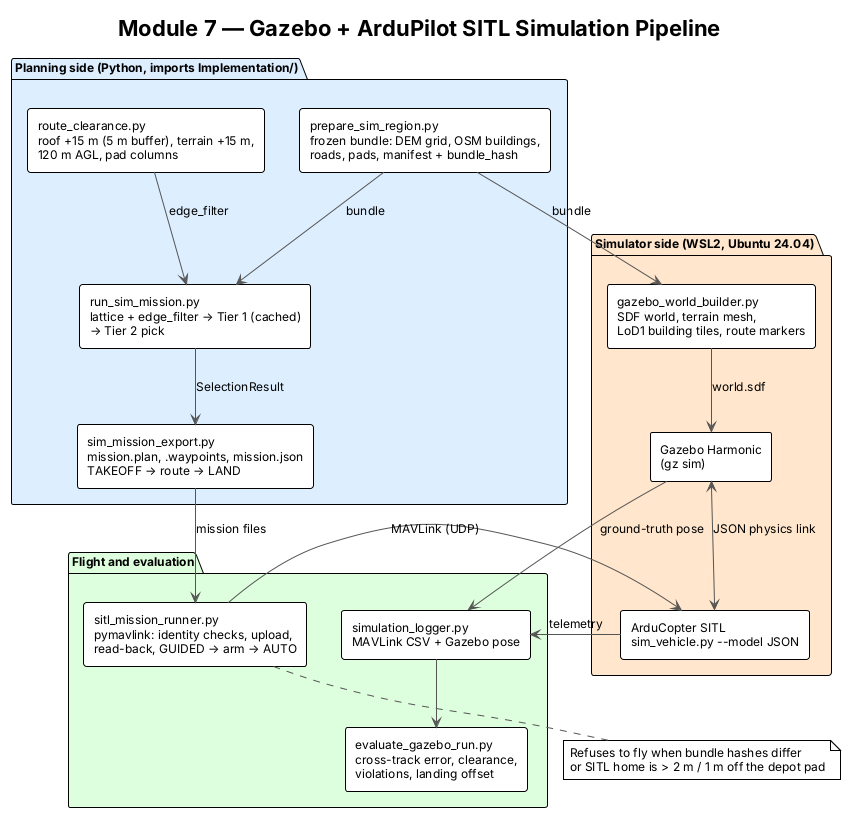
\includegraphics[width=\textwidth,height=0.28\textheight,keepaspectratio]{images/simulation.png}
\caption{Gazebo and ArduPilot SITL simulation pipeline}\label{fig:sim}
\end{figure}

\subsection{Bundle, clearance and frame contract}

A region is first frozen into a bundle: a terrain grid, OSM buildings with heights,
roads, the depot and destination pads, and a manifest. Its hash is written into the
graph, the front, the mission file and the world, and the runner refuses to fly if they
do not match. Before NAMOA* runs, a clearance checker passed in as \texttt{edge\_filter}
removes every edge that passes less than 15\,m above a buffered roof or the terrain, or
goes above 120\,m above ground. The Gazebo world has its origin at the depot pad, where
SITL also places home, so a mission altitude means the same height in the planner, the
world and the autopilot.

\subsection{Mission sequence}

Figure~\ref{fig:sequence} follows one mission from the operator's tags to the flown
route. Tier~1 runs only when the stored front is stale or missing. Tier~2 then returns
either a HOLD advisory or a selection that is exported as a mission file. The runner uploads and reads back the mission, arms, switches to AUTO and
logs telemetry until landing. An evaluator then computes the cross-track error, the
minimum clearance, any rule breach and the landing offset from the pad.

\begin{figure}[!htbp]
\centering
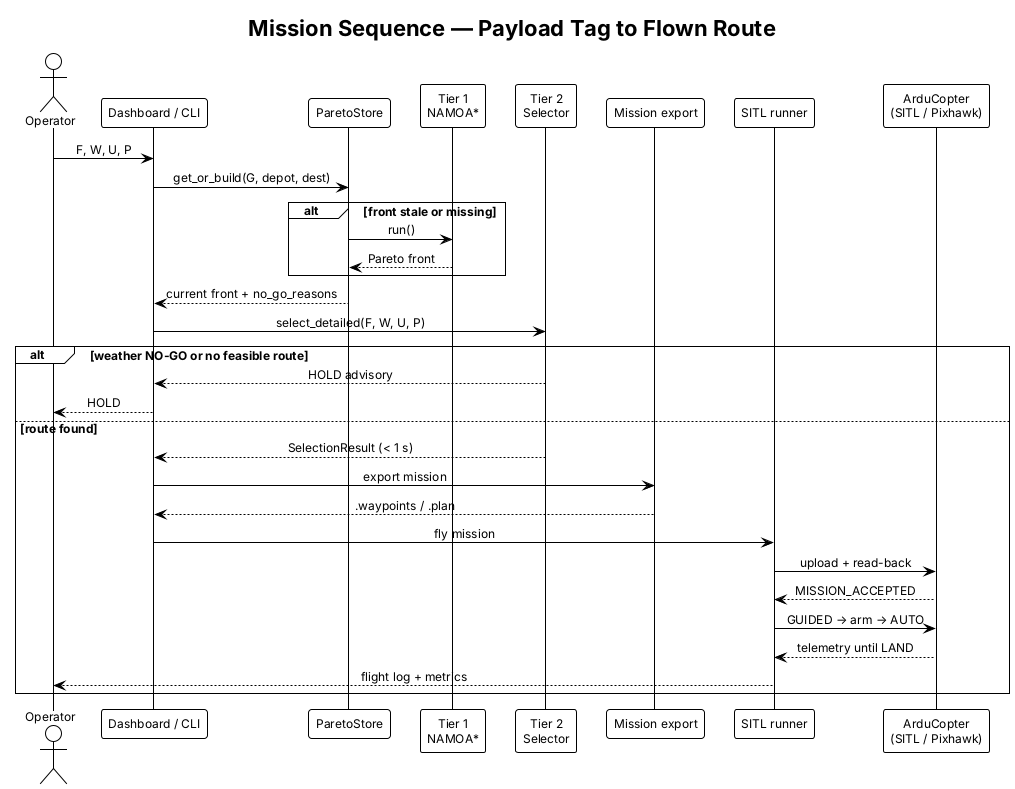
\includegraphics[width=0.72\textwidth]{images/mission_sequence.png}
\caption{Mission sequence from payload tag entry to the flown route}\label{fig:sequence}
\end{figure}
